Un rectangle té dos vèrtexs sobre l'eix d'abscisses i els altres dos sobre la paràbola
$y=12-x^2$, tal com es pot veure a la figura. Anomenem $x$ la meitat de la base.

\begin{center}
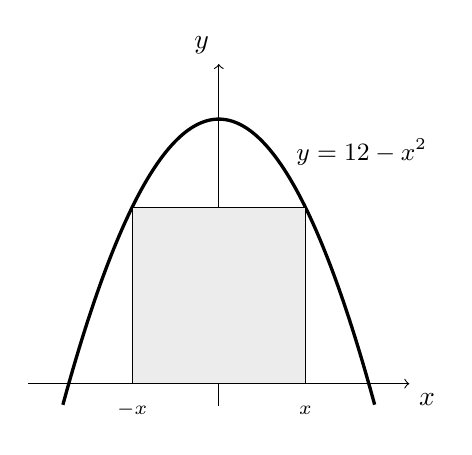
\begin{tikzpicture}[x=0.55cm,y=0.28cm]
  \draw[->] (-4.4,0) -- (4.4,0) node[below right] {$x$};
  \draw[->] (0,-1) -- (0,14.5) node[above left] {$y$};
  \draw[\colorgrafica,very thick,domain=-3.6:3.6,samples=80,smooth] plot (\x,{12-\x*\x});
  \draw[fill=gray!15] (-2,0) rectangle (2,8);
  \node[font=\scriptsize] at (2,-1.2) {$x$};
  \node[font=\scriptsize] at (-2,-1.2) {$-x$};
  \node[\colorgrafica,font=\small] at (3.3,10.5) {$y=12-x^2$};
\end{tikzpicture}
\end{center}

\begin{apartats}

\apartat[1,25]{1}
Comprova que l'àrea del rectangle és $A(x)=24x-2x^3$ i digues entre quins valors pot variar
$x$.

\begin{solucio}
La base fa $2x$ i l'altura és l'ordenada de la paràbola, $12-x^2$. Per tant,
\[
A(x)=2x\left(12-x^2\right)=24x-2x^3 .
\]
Perquè el rectangle existeixi cal $x>0$ i $12-x^2>0$: $x\in\left(0,\sqrt{12}\right)$.
\end{solucio}

\apartat[1,25]{0,75}
Troba el valor de $x$ que fa màxima l'àrea i calcula aquesta àrea.

\begin{solucio}
$A'(x)=24-6x^2=0\iff x^2=4\iff x=2$ (l'altra solució, $x=-2$, no és al domini).\\
$A(2)=48-16=32$: el rectangle fa $4$ de base i $8$ d'altura, i l'àrea màxima és
$\boxed{32}$ unitats quadrades.
\end{solucio}

\begin{nomesllarg}
\apartat{0,75}
Justifica, amb la derivada segona, que el valor trobat dona un màxim.

\begin{solucio}
$A''(x)=-12x$, i $A''(2)=-24<0$: la funció és còncava en $x=2$, i per tant hi ha un
\textbf{màxim}.\\
També es veu pel signe de $A'$: positiva a $(0,2)$ i negativa a $\left(2,\sqrt{12}\right)$.
\end{solucio}
\end{nomesllarg}

\end{apartats}
